\documentclass[11pt]{article}
\usepackage{amsgen,amsmath,amstext,amsbsy,amsopn,amssymb}
%\usepackage[dvips]{graphicx,color}
\usepackage{graphicx,color}
\usepackage{graphicx,color,bm}
\usepackage{epsfig}
\usepackage{enumerate}
\usepackage{float}

%\setlength{\oddsidemargin}{0.1 in} \setlength{\evensidemargin}{-0.1
%in} \setlength{\topmargin}{-0.6 in} \setlength{\textwidth}{6.5 in}
%\setlength{\textheight}{8.5 in} \setlength{\headsep}{0.75 in}
%\setlength{\parindent}{0 in} \setlength{\parskip}{0.1 in}

\textwidth 6.3in \textheight 8.8in \topmargin -0.5truein
\oddsidemargin .15truein
\parskip .1in
\renewcommand{\baselinestretch}{1.53}  % double spaced


\newcommand{\homework}[9]{
	\pagestyle{myheadings}
	\thispagestyle{plain}
	\newpage
	\setcounter{page}{1}
	\noindent
	\begin{center}
		\framebox{
			\vbox{\vspace{2mm}
				\hbox to 6.28in { {\bf Math531:~Regression - I  \hfill} }
				\vspace{6mm}
				\hbox to 6.28in { {\Large \hfill #1 (#2)  \hfill} }
				\vspace{6mm}
				\hbox to 6.28in { {\it Instructor: #3 \hfill} }
				\hbox to 6.28in { {\it Office hours: #4  \hfill #6}}
				\vspace{2mm}}
		}
	\end{center}
	\markboth{#1}{#1}
	\vspace*{4mm}
}

% ----------------------- MATH -------------------------
\def\av{\boldsymbol a}
\def\bv{\boldsymbol b}
\def\cv{\boldsymbol c}
\def\dv{\boldsymbol d}
\def\ev{\boldsymbol e}
\def\fv{\boldsymbol f}
\def\gv{\boldsymbol g}
\def\hv{\boldsymbol h}
\def\iv{\boldsymbol i}
\def\gv{\boldsymbol j}
\def\kv{\boldsymbol k}
\def\lv{\boldsymbol l}
\def\mv{\boldsymbol m}
\def\nv{\boldsymbol n}
\def\ov{\boldsymbol o}
\def\pv{\boldsymbol p}
\def\qv{\boldsymbol q}
\def\rv{\boldsymbol r}
\def\sv{\boldsymbol s}
\def\tv{\boldsymbol t}
\def\uv{\boldsymbol u}
\def\vv{\boldsymbol v}
\def\wv{\boldsymbol w}
\def\xv{\boldsymbol x}
\def\yv{\boldsymbol y}
\def\zv{\boldsymbol z}
\def\Av{\boldsymbol A}
\def\Bv{\boldsymbol B}
\def\Cv{\boldsymbol C}
\def\Dv{\boldsymbol D}
\def\Ev{\boldsymbol E}
\def\Fv{\boldsymbol F}
\def\Gv{\boldsymbol G}
\def\Hv{\boldsymbol H}
\def\Iv{\boldsymbol I}
\def\Gv{\boldsymbol J}
\def\Kv{\boldsymbol K}
\def\Lv{\boldsymbol L}
\def\Mv{\boldsymbol M}
\def\Nv{\boldsymbol N}
\def\Ov{\boldsymbol O}
\def\Pv{\boldsymbol P}
\def\Qv{\boldsymbol Q}
\def\Rv{\boldsymbol R}
\def\Sv{\boldsymbol S}
\def\Tv{\boldsymbol T}
\def\Uv{\boldsymbol U}
\def\Vv{\boldsymbol V}
\def\Wv{\boldsymbol W}
\def\Xv{\boldsymbol X}
\def\Yv{\boldsymbol Y}
\def\Zv{\boldsymbol Z}
\def\Abf{\mathbf A}
\def\Bbf{\mathbf B}
\def\Cbf{\mathbf C}
\def\Dbf{\mathbf D}
\def\Ebf{\mathbf E}
\def\Fbf{\mathbf F}
\def\Gbf{\mathbf G}
\def\Hbf{\mathbf H}
\def\Ibf{\mathbf I}
\def\Gbf{\mathbf J}
\def\Kbf{\mathbf K}
\def\Lbf{\mathbf L}
\def\Mbf{\mathbf M}
\def\Nbf{\mathbf N}
\def\Obf{\mathbf O}
\def\Pbf{\mathbf P}
\def\Qbf{\mathbf Q}
\def\Rbf{\mathbf R}
\def\Sbf{\mathbf S}
\def\Tbf{\mathbf T}
\def\Ubf{\mathbf U}
\def\Vbf{\mathbf V}
\def\Wbf{\mathbf W}
\def\Xbf{\mathbf X}
\def\Ybf{\mathbf Y}
\def\Jbf{\mathbf J}
\def\Zbf{\mathbf Z}
\def\Am{\mathrm A}
\def\Bm{\mathrm B}
\def\Cm{\mathrm C}
\def\Dm{\mathrm D}
\def\Em{\mathrm E}
\def\Fm{\mathrm F}
\def\Gm{\mathrm G}
\def\Hm{\mathrm H}
\def\Im{\mathrm I}
\def\Gm{\mathrm J}
\def\Km{\mathrm K}
\def\Lm{\mathrm L}
\def\Mm{\mathrm M}
\def\Nm{\mathrm N}
\def\Om{\mathrm O}
\def\Pm{\mathrm P}
\def\Qm{\mathrm Q}
\def\Rm{\mathrm R}
\def\Sm{\mathrm S}
\def\Tm{\mathrm T}
\def\Um{\mathrm U}
\def\mv{\mathrm V}
\def\Wm{\mathrm W}
\def\Xm{\mathrm X}
\def\Ym{\mathrm Y}
\def\Zm{\mathrm Z}
\newcommand{\Ac}{\mathcal{A}}
\newcommand{\Bc}{\mathcal{B}}
\newcommand{\Cc}{\mathcal{C}}
\newcommand{\Dc}{\mathcal{D}}
\newcommand{\Ec}{\mathcal{E}}
\newcommand{\Fc}{\mathcal{F}}
\newcommand{\Gc}{\mathcal{G}}
\newcommand{\Hc}{\mathcal{H}}
\newcommand{\Ic}{\mathcal{I}}
\newcommand{\Jc}{\mathcal{J}}
\newcommand{\Kc}{\mathcal{K}}
\newcommand{\Lc}{\mathcal{L}}
\newcommand{\Mc}{\mathcal{M}}
\newcommand{\Nc}{\mathcal{N}}
\newcommand{\Oc}{\mathcal{O}}
\newcommand{\Pc}{\mathcal{P}}
\newcommand{\Qc}{\mathcal{Q}}
\newcommand{\Rc}{\mathcal{R}}
\newcommand{\Sc}{\mathcal{S}}
\newcommand{\Tc}{\mathcal{T}}
\newcommand{\Uc}{\mathcal{U}}
\newcommand{\Vc}{\mathcal{V}}
\newcommand{\Wc}{\mathcal{W}}
\newcommand{\Xc}{\mathcal{X}}
\newcommand{\Yc}{\mathcal{Y}}
\newcommand{\Zc}{\mathcal{Z}}
\newcommand{\alphav}{\mbox{\boldmath{$\alpha$}}}
\newcommand{\betav}{\mbox{\boldmath{$\beta$}}}
\newcommand{\gammav}{\mbox{\boldmath{$\gamma$}}}
\newcommand{\deltav}{\mbox{\boldmath{$\delta$}}}
\newcommand{\epsilonv}{\mbox{\boldmath{$\epsilon$}}}
\newcommand{\zetav}{\mbox{\boldmath$\zeta$}}
\newcommand{\etav}{\mbox{\boldmath{$\eta$}}}
\newcommand{\iotav}{\mbox{\boldmath{$\iota$}}}
\newcommand{\kappav}{\mbox{\boldmath{$\kappa$}}}
\newcommand{\lambdav}{\mbox{\boldmath{$\lambda$}}}
\newcommand{\muv}{\mbox{\boldmath{$\mu$}}}
\newcommand{\nuv}{\mbox{\boldmath{$\nu$}}}
\newcommand{\xiv}{\mbox{\boldmath{$\xi$}}}
\newcommand{\omicronv}{\mbox{\boldmath{$\omicron$}}}
\newcommand{\piv}{\mbox{\boldmath{$\pi$}}}
\newcommand{\rhov}{\mbox{\boldmath{$\rho$}}}
\newcommand{\sigmav}{\mbox{\boldmath{$\sigma$}}}
\newcommand{\tauv}{\mbox{\boldmath{$\tau$}}}
\newcommand{\upsilonv}{\mbox{\boldmath{$\upsilon$}}}
\newcommand{\phiv}{\mbox{\boldmath{$\phi$}}}
\newcommand{\varphiv}{\mbox{\boldmath{$\varphi$}}}
\newcommand{\chiv}{\mbox{\boldmath{$\chi$}}}
\newcommand{\psiv}{\mbox{\boldmath{$\psi$}}}
\newcommand{\omegav}{\mbox{\boldmath{$\omega$}}}
\newcommand{\Sigmav}{\mbox{\boldmath{$\Sigma$}}}
\newcommand{\Lambdav}{\mbox{\boldmath{$\Lambda$}}}
\newcommand{\Deltav}{\mbox{\boldmath{$\Delta$}}}
\newcommand{\Omegav}{\mbox{\boldmath{$\Omega$}}}
\newcommand{\varepsilonv}{\mbox{\boldmath{$\varepsilon$}}}

\newcommand{\eps}{\varepsilon}
\newcommand{\epsv}{\mbox{\boldmath{$\varepsilon$}}}

\def\1v{\mathbf 1}
\def\0v{\mathbf 0}
\def\Id{\mathbf I} % identity matrix
\newcommand{\ind}[1]{\mathbbm{1}_{\left[ {#1} \right] }}
\newcommand{\Ind}[1]{\mathbbm{1}_{\left\{ {#1} \right\} }}
\newcommand\indep{\protect\mathpalette{\protect\independenT}{\perp}}\def\independenT#1#2{\mathrel{\rlap{$#1#2$}\mkern2mu{#1#2}}}
\newcommand{\QED}{\begin{flushright} {\bf QED} \end{flushright}}
\newcommand{\R}{\mathbb R}
\newcommand{\Real}{\mathbb R}
\newcommand{\C}{\mathbb C}
\newcommand{\E}{\mathbb E}
\newcommand{\sgn}{\mathop{\mathrm{sign}}}
\def\Pr{\mathrm P}
\def\pr{\mathrm P}
\newcommand{\Var}{\mathop{\rm Var}}
\newcommand{\var}{\mathop{\rm Var}}
\newcommand{\Cov}{\mathop{\rm Cov}}
\newcommand{\cov}{\mathop{\rm Cov}}
\newcommand{\Corr}{\mathop{\rm Corr}}
\newcommand{\ang}{\mathop{\rm Angle}}
\newcommand{\tr}{\mathop{\rm trace}}
\newcommand{\proj}{\mathop{\rm Proj}}
\newcommand{\rank}{\mathop{\rm rank}}

\newcommand{\diag}{\mathop{\rm diag}}
\newcommand{\Diag}{\mathop{\rm diag}}
\newcommand{\sk}{\vspace{0.5cm}}
\newcommand{\ds}{\displaystyle}
\newcommand{\mb}{\mbox}
\newcommand{\wh}{\widehat}
\newcommand{\argmin}{\operatornamewithlimits{argmin}}
\newcommand{\argmax}{\operatornamewithlimits{argmax}}

\newcommand{\norm}[1]{\|#1\|}
\newcommand{\abs}[1]{\left\vert#1\right\vert}
\newcommand{\set}[1]{\left\{#1\right\}}

\newcommand{\To}{\longrightarrow}

\def\equalLaw{\stackrel{\mathcal{L}}{=}}
\def\equallaw{\stackrel{\mathcal{L}}{=}}

\def\half{\frac{1}{2}}

\usepackage{caption}

\begin{document}

\begin{title}
	{\Large\bf Homework 7, MATH 455: Due Mon, 04/30/2018}
\end{title}

\author{\bf Alexander Van Roijen}

\maketitle
{\bf Instructions}:  The homework assignment editing this \LaTeX\ document.  Download the \LaTeX\ source from the class web page and study
it to learn more about \LaTeX.  Replace the text with appropriate information.  Run ``pdflatex'' on this document.

You will submit this assignment in two parts:
\begin{enumerate}
\item Print out the PDF file and bring it to class, and
\item Send an e-mail to:
\begin{center}
gang@math.binghamton.edu
\end{center}
\emph{before class} on the due date with two attachments:
\begin{itemize}
\item The \LaTeX\ source file, and
\item The generated PDF document.
\end{itemize}
\end{enumerate}
\newpage
Please complete the following:
\begin{enumerate}
\item  Finish R exercises 11.1, 11.2, 11.3, 11.4, 11.6 of the textbook. Submit your answers for {\color{red}ALL} questions.
\begin{enumerate}
	\item 11.1
	We first take a look at the PC
	\begin{verbatim}
		> hold=prcomp(seatpos[,-c(9,1,2)])
		> print(summary(hold))
		Importance of components:
		PC1     PC2     PC3     PC4     PC5     PC6
		Standard deviation     17.1573 2.89689 2.11907 1.56412 1.22502 0.46218
		Proportion of Variance  0.9453 0.02695 0.01442 0.00786 0.00482 0.00069
		Cumulative Proportion   0.9453 0.97222 0.98664 0.99450 0.99931 1.00000
	\end{verbatim}
	Looks like the first two components explain most of the variation of our data.
	Using them for our prediction we get the following.
	\begin{verbatim}
		> cmonnow = pcr(hipcenter~.-Age-Weight,data=seatpos[],ncomp=2)
		> predict(cmonnow,testhcf,ncomp=2,interval="prediction")
		, , 2 comps
		
		hipcenter
		1 -204.4636
	\end{verbatim}
	\item 11.2
	We fit a partial least squares model to the same data and examine the number of components to use.
		\begin{figure}[H]
			\centering
			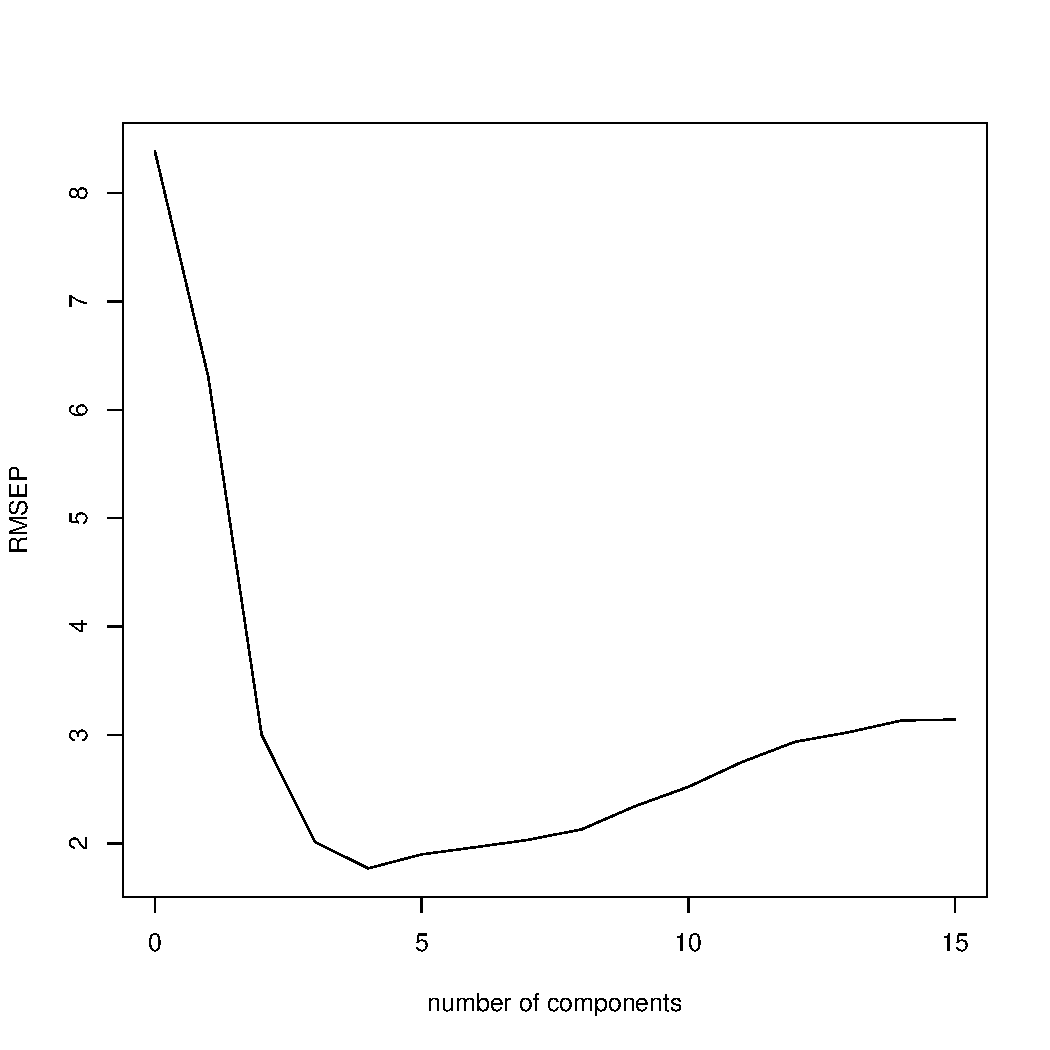
\includegraphics[width=10cm,height=10cm]{112numc.pdf}
			\caption[paic]{examining the residual mean squared error over number of components and choosing the min value}
			\label{cspos}
		\end{figure}
		we then use 4 components as it has the minmum RMSEP value and we get teh following prediction
		\begin{verbatim}
			> splsmod <- plsr(hipcenter ~ ., data=seatpos, validation="CV")
			> #4 components looks good
			> hcpred = predict(splsmod,testhcf,ncomp=4)
			> print(hcpred)
			, , 4 comps
			
			hipcenter
			1 -179.4634
		\end{verbatim}
	\item 11.3
	We are now going to fit a ridge regression model to the seatpos data
	\begin{figure}[H]
		\centering
		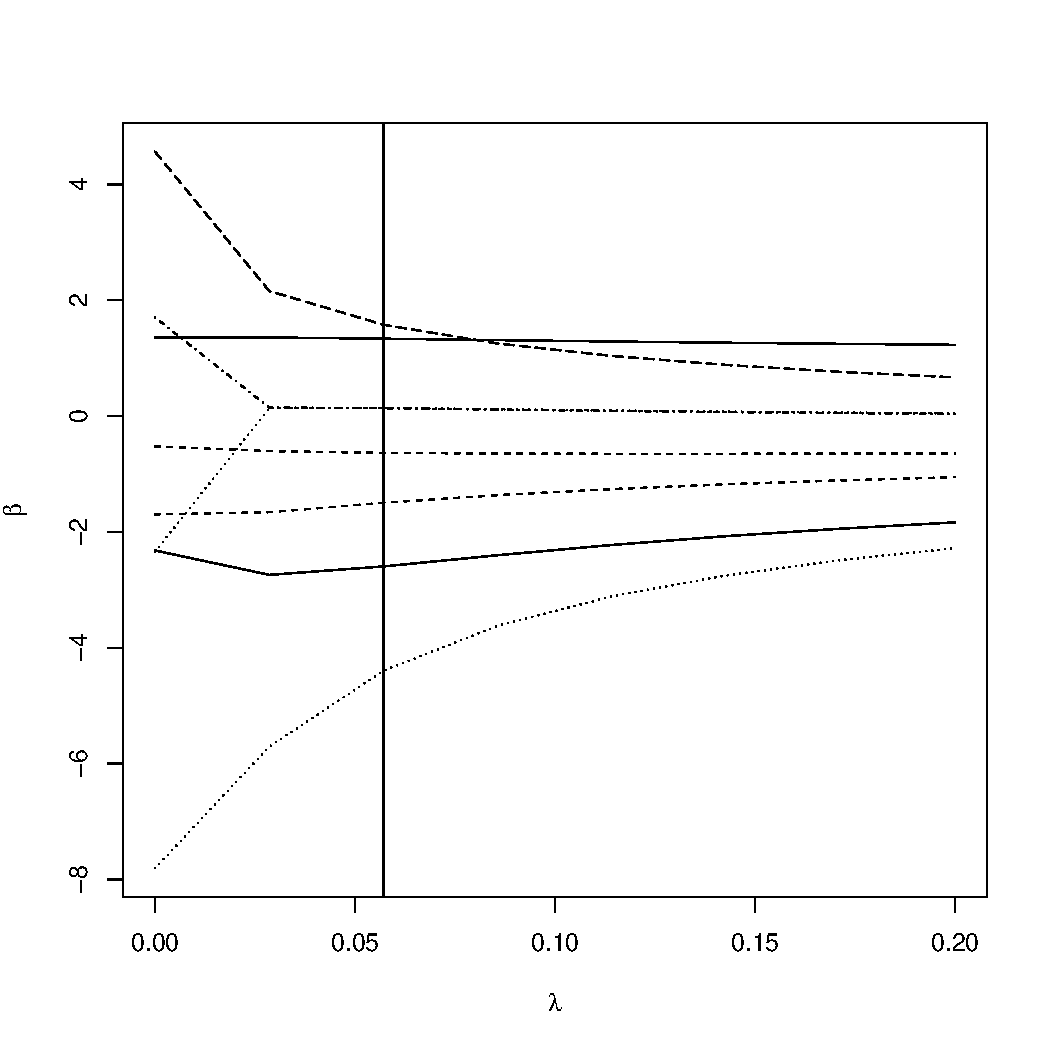
\includegraphics[width=10cm,height=10cm]{hcrgp.pdf}
		\caption[paic]{examining th}
		\label{hcrgp}
	\end{figure}
	using the minimum lambda value provided of ~0.05, we get the following prediction
	\begin{verbatim}
		> hcrgpred1 = cbind(1,as.matrix(testhcf[1,]))%*%coef(hcrgmod2)[8,]
		> hcrgpred1
		[,1]
		1 -175.488
	\end{verbatim}
	\item 11.4\\
	We first remove each tenth observation and seperate the data.
	\begin{verbatim}
		fat2=fat[-seq(1,length(fat[,1]),10),]
		testfat = fat[seq(1,length(fat[,1]),10),]
	\end{verbatim} 
	\begin{enumerate}
		\item a
		we now fit a linear model and get the following prediction accuracy described by the residual mean squared error between the predictions and the actual observations
		\begin{verbatim}
			> oglg = lm(siri ~ . -brozek -density,fat2)
			> wut=predict(oglg,newdata=testfat)
			> rmse(wut,testfat$siri)
			[1] 1.946023
		\end{verbatim}
		\item b
		we now use the stepwise function to determine the "ideal" model 
		\begin{verbatim}
			> stepwise(lm(siri ~ . -brozek -density,fat2),criterion = c("AIC"),direction=c("forward"))
			Call:
			lm(formula = siri ~ abdom + free + weight + forearm + adipos + 
			thigh + chest + biceps + ankle, data = fat2)
			
			Coefficients:
			(Intercept)        abdom         free       weight      forearm       adipos        thigh        chest       biceps  
			-2.9190       0.1179      -0.5698       0.3925       0.2146      -0.5277       0.1561       0.1246       0.1490  
			ankle  
			0.1475  
		\end{verbatim}
		I chose forward progression, and proceeded to fit a model with the chosen parameters and got the following prediction results
		\begin{verbatim}
			> splg = lm(formula = siri ~ abdom + free + weight + forearm + adipos + thigh + chest + biceps + ankle, data = fat2)
			> wut2=predict(splg,newdata=testfat)
			> rmse(wut2,testfat$siri)
			[1] 1.98911
		\end{verbatim}
		we see a slightly higher RMSE, but overall quite close and simpler too
		\item c
		Now we want to fit a principle component regression onto our data.
		\begin{verbatim}
			> print(summary(temp))
			Importance of components:
			PC1     PC2      PC3     PC4     PC5     PC6     PC7     PC8     PC9    PC10    PC11    PC12
			Standard deviation     36.8986 15.5341 10.29573 3.66009 3.44451 2.64961 2.14660 1.88702 1.57469 1.43989 1.30247 1.21438
			Proportion of Variance  0.7736  0.1371  0.06023 0.00761 0.00674 0.00399 0.00262 0.00202 0.00141 0.00118 0.00096 0.00084
			Cumulative Proportion   0.7736  0.9107  0.97095 0.97856 0.98531 0.98929 0.99191 0.99394 0.99534 0.99652 0.99749 0.99832
			PC13    PC14    PC15    PC16
			Standard deviation     1.06850 1.00511 0.75913 0.46948
			Proportion of Variance 0.00065 0.00057 0.00033 0.00013
			Cumulative Proportion  0.99897 0.99955 0.99987 1.00000
		\end{verbatim}
		I choose to only include the first 3 PRC as they cover about 97 percent of the variation in the data.\\
		Fitting the model, we now get
		\begin{verbatim}
			> fatpcr = pcr(siri ~ . -brozek -density,data=fat2,ncomp=3)
			> pcrr= predict(fatpcr,testfat,ncomp=3,interval="prediction")
			> rmse(pcrr,testfat$siri)
			[1] 2.487871
		\end{verbatim}
		the RMSE is quite higher, looking at a PCR with all PCs we get
		\begin{verbatim}
			> rmse(pcrr2,testfat$siri)
			[1] 1.946023
		\end{verbatim}
		so we could improve our RMSE, but that would effectively negate the point of PCR.
		\item d
		Looking at a partial least squares regression, we create the following
			\begin{figure}[H]
				\centering
				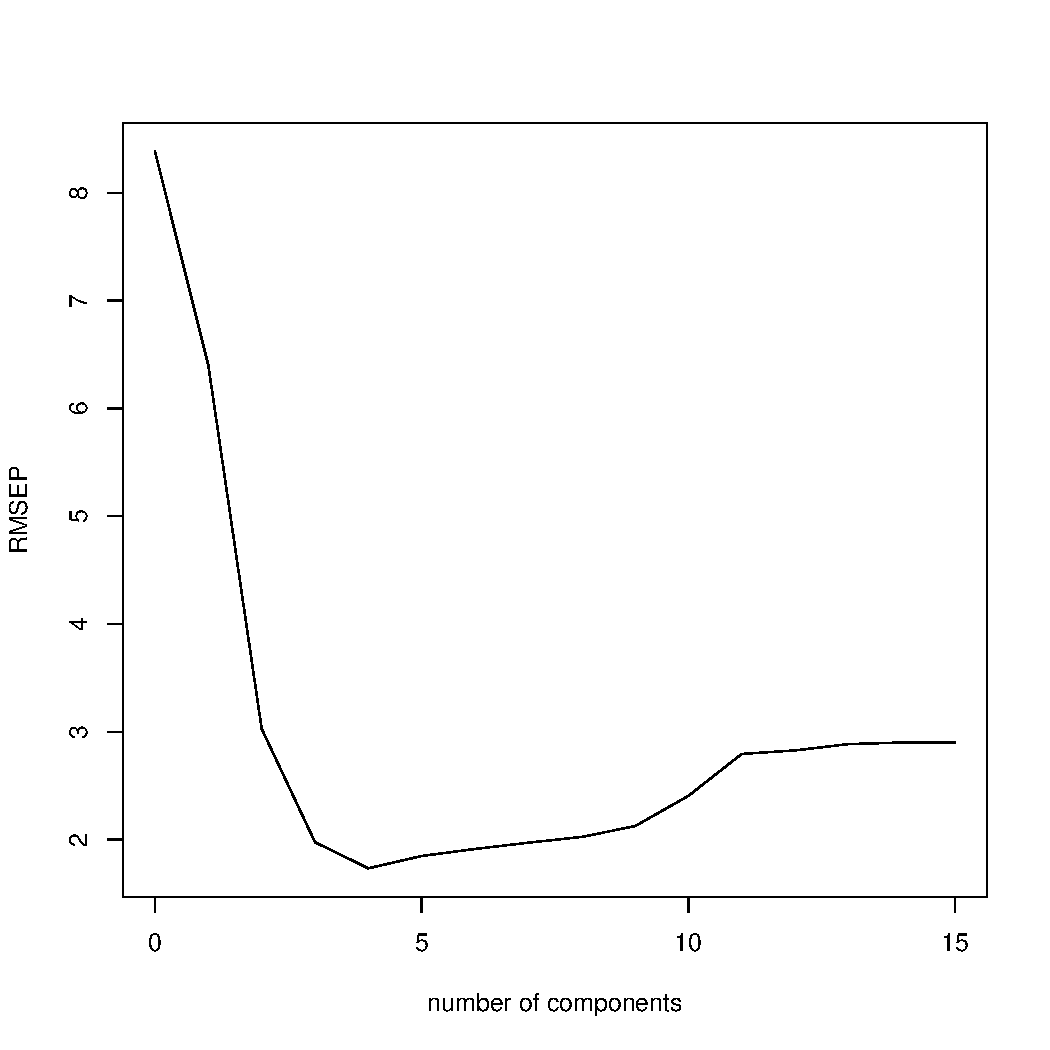
\includegraphics[width=10cm,height=10cm]{114dc.pdf}
				\caption[paic]{a look at at the ideal number of components for our PLSR}
				\label{plsr}
			\end{figure}
		We determine graphically and within the code that 4 components is the ideal choice. We achieve the following.
		\begin{verbatim}
			> summary(fatpls)
			Data: 	X dimension: 226 15 
			Y dimension: 226 1
			Fit method: kernelpls
			Number of components considered: 15
			
			VALIDATION: RMSEP
			Cross-validated using 10 random segments.
			(Intercept)  1 comps  2 comps  3 comps  4 comps  5 comps  6 comps  7 comps  8 comps  9 comps  10 comps  11 comps
			CV           8.382    6.384    2.998    1.967    1.709    1.822    1.889    1.955    2.041    2.231     2.658     2.738
			adjCV        8.382    6.379    2.997    1.962    1.698    1.800    1.858    1.920    1.998    2.174     2.571     2.646
			12 comps  13 comps  14 comps  15 comps
			CV        2.848     2.906     2.944     2.952
			adjCV     2.749     2.804     2.839     2.846
			
			TRAINING: % variance explained
			1 comps  2 comps  3 comps  4 comps  5 comps  6 comps  7 comps  8 comps  9 comps  10 comps  11 comps  12 comps
			X       76.85    90.81    97.13    97.83    98.24    98.54    99.04    99.27    99.40     99.49     99.60     99.67
			siri    44.30    87.73    95.02    96.72    96.94    97.07    97.11    97.14    97.15     97.16     97.16     97.16
			13 comps  14 comps  15 comps
			X        99.83     99.92    100.00
			siri     97.16     97.16     97.16
			> hcpred = predict(fatpls,testfat,ncomp=4)
			> rmse(hcpred,testfat$siri)
			[1] 1.973459
		\end{verbatim}
		Similar predictive ability to other models we have seen
		\item e
		Ridge regression! Exciting stuff, this bad boy will let us trim down the size of our model a bit by utilizing a penalty term! Lets examine the potentials of this idea.
			\begin{figure}[H]
				\centering
				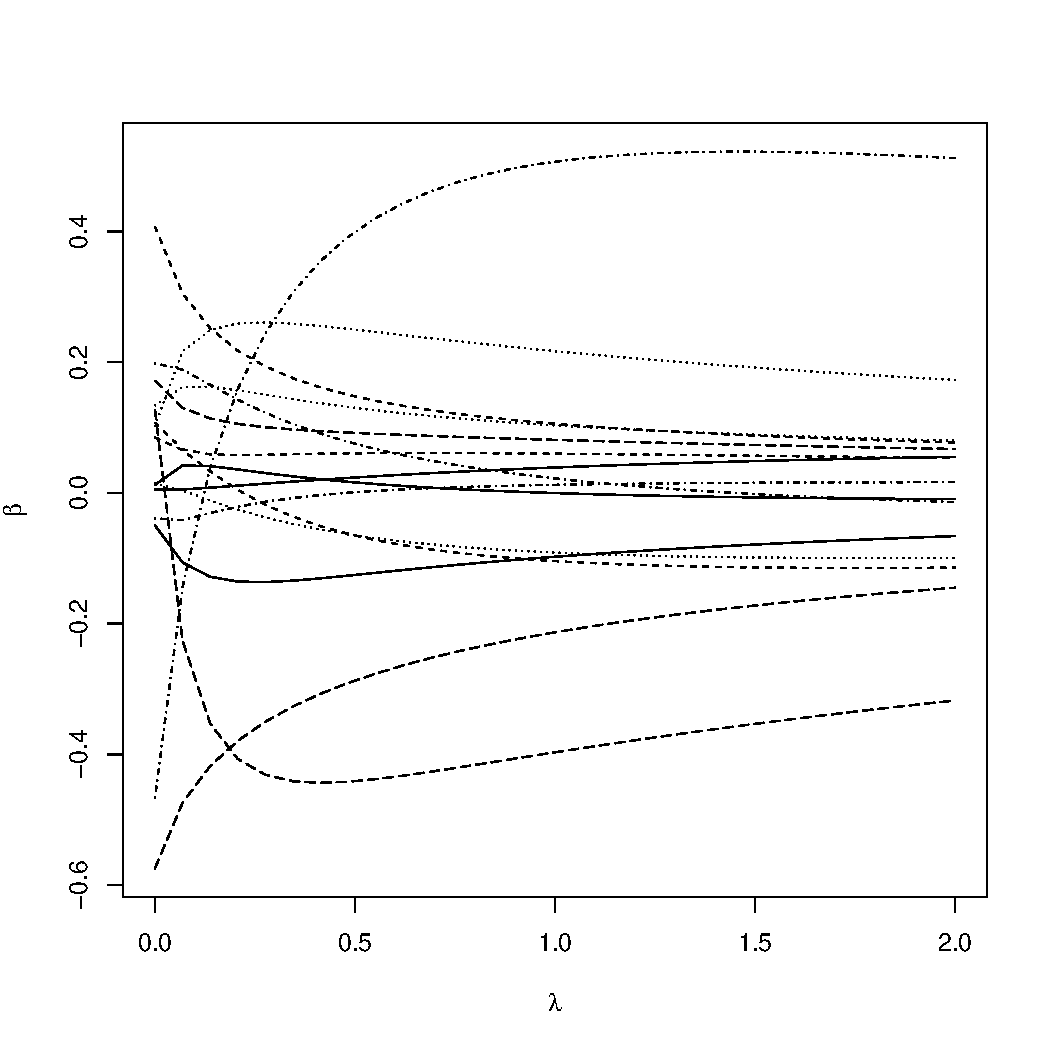
\includegraphics[width=10cm,height=10cm]{fatrgp.pdf}
				\caption[fr]{a look at at the ideal number of components for our PLSR}
				\label{fatridge}
			\end{figure}
			This is hard to interpret, so lets analyze the minimum GCV to get an idea of what our penalty term should be.
			\begin{verbatim}
				> fatrm = lm.ridge(siri ~ .-brozek -density,data=fat2,lambda=seq(0,2,len=30))
				> which.min(fatrm$GCV)
				0.00000000 
				1 
			\end{verbatim}
			This zero implies that our best bet is zero penalty, which equivalently that reducing the model provides no optimization here and the OLS is best. We find that the RMSE is the same as our OLS in part a, which coincides with our thoughts.
			\begin{verbatim}
				> hcrgpred1 = cbind(1,as.matrix(rmtestfat))%*%(coef(fatrm)[1,])
				> rmse(hcrgpred1,testfat$siri)
				[1] 1.946023
			\end{verbatim}
	\end{enumerate}
	\item 11.6
	\begin{enumerate}
		\item a
		\begin{verbatim}
			> withoutData=kanga[complete.cases(kanga),]
			> withoutData$sex = as.numeric(as.factor(withoutData$sex))
			> withoutData$species = as.numeric(as.factor(withoutData$species))
			> temp = prcomp(withoutData)
			> print(summary(temp))
			Importance of components:
			Importance of components:
			PC1      PC2      PC3      PC4      PC5      PC6      PC7     
			Standard deviation     288.0383 69.51358 30.74721 27.85652 21.73040 19.42447 17.28302 
			Proportion of Variance   0.9002  0.05243  0.01026  0.00842  0.00512  0.00409  0.00324  
			Cumulative Proportion    0.9002  0.95268  0.96294  0.97136  0.97648  0.98058  0.98382  
		\end{verbatim}
		As we can see, our first principal component covers 90 percent of variation
		\item b
		\begin{verbatim}
			> print(temp$rotation[,1])
			species                  sex       basilar.length occipitonasal.length        palate.length 
			-9.470452e-05        -6.133600e-04        -4.840682e-01        -4.562961e-01        -3.662141e-01 
			palate.width         nasal.length          nasal.width      squamosal.depth       lacrymal.width 
			-8.435755e-02        -2.480989e-01        -7.464748e-02        -6.366132e-02        -1.189368e-01 
			zygomatic.width        orbital.width       .rostral.width      occipital.depth          crest.width 
			-2.066976e-01        -1.428888e-02        -1.064589e-01        -1.781770e-01         8.196805e-02 
			foramina.length      mandible.length       mandible.width       mandible.depth         ramus.height 
			-9.941184e-03        -4.359818e-01        -2.999679e-02        -5.832212e-02        -2.090714e-01 
		\end{verbatim}
		As we can see, mandible length, occipitonasal length, palate length, and basilar length are the prominent terms
		\item c
		\begin{verbatim}
			> temp2 = prcomp(withoutData,scale=TRUE)
			> print(summary(temp2))
			Importance of components:
			PC1    PC2     PC3     PC4     PC5     PC6     PC7     PC8    ...
			Standard deviation     3.5509 1.5178 1.11386 1.00232 0.84943 0.69411 0.55590 0.51277 ....
			Proportion of Variance 0.6304 0.1152 0.06203 0.05023 0.03608 0.02409 0.01545 0.01315 ....
			Cumulative Proportion  0.6304 0.7456 0.80765 0.85788 0.89396 0.91805 0.93350 0.94665 ...
		\end{verbatim}
		We can tell that, similar to the fat data set we analyzed in class, there is a leveled out effect. Large values are made less significant and thus the proportion of variance per component is less prominent.
		\item d
		\begin{verbatim}
			> print(temp2$rotation[,1])
			species                  sex       basilar.length occipitonasal.length        palate.length 0.27531510           0.26524013           0.27393581 
			palate.width         nasal.length          nasal.width      squamosal.depth       lacrymal.width 
			0.23270782           0.22767199           0.22577402           0.23719817           0.26469478 
			zygomatic.width        orbital.width       .rostral.width      occipital.depth          crest.width 
			0.25677431           0.07539545           0.25588530           0.26958527          -0.16377366 
			foramina.length      mandible.length       mandible.width       mandible.depth         ramus.height 
			0.05683491           0.27711781           0.20971711           0.23837398           0.25841572 
			> print(temp2$rotation[,2])
			species                  sex       basilar.length occipitonasal.length        palate.length 
			0.5649159512        -0.0459169262         0.0090950112         0.1659461872         0.0504494218 
			palate.width         nasal.length          nasal.width      squamosal.depth       lacrymal.width 
			0.0121999313         0.3258713200         0.2396642898        -0.1554982206         0.0291972986 
			zygomatic.width        orbital.width       .rostral.width      occipital.depth          crest.width 
			-0.2214711336         0.0502588495         0.0007699419        -0.0243930064        -0.3420526961 
			foramina.length      mandible.length       mandible.width       mandible.depth         ramus.height 
			0.3370527404        -0.0189223029        -0.3231510620        -0.2003645746        -0.1791012252 
		\end{verbatim}
		the second PC shows a strong correlation with species, crest width, nasal length, and formalin length. The first one represented that a lot of these kangaroos are a lot more similar, while the second PC, orthogonal to the first, shows that they differ in the corresponding high valued components. We can see this mainly some higher values, like .33 for foramina length in the second PC. Unlike the first, it is not as level, and thus different components \textbf{differentiate} the kangaroos
		\item e
		\begin{figure}[H]
			\centering
			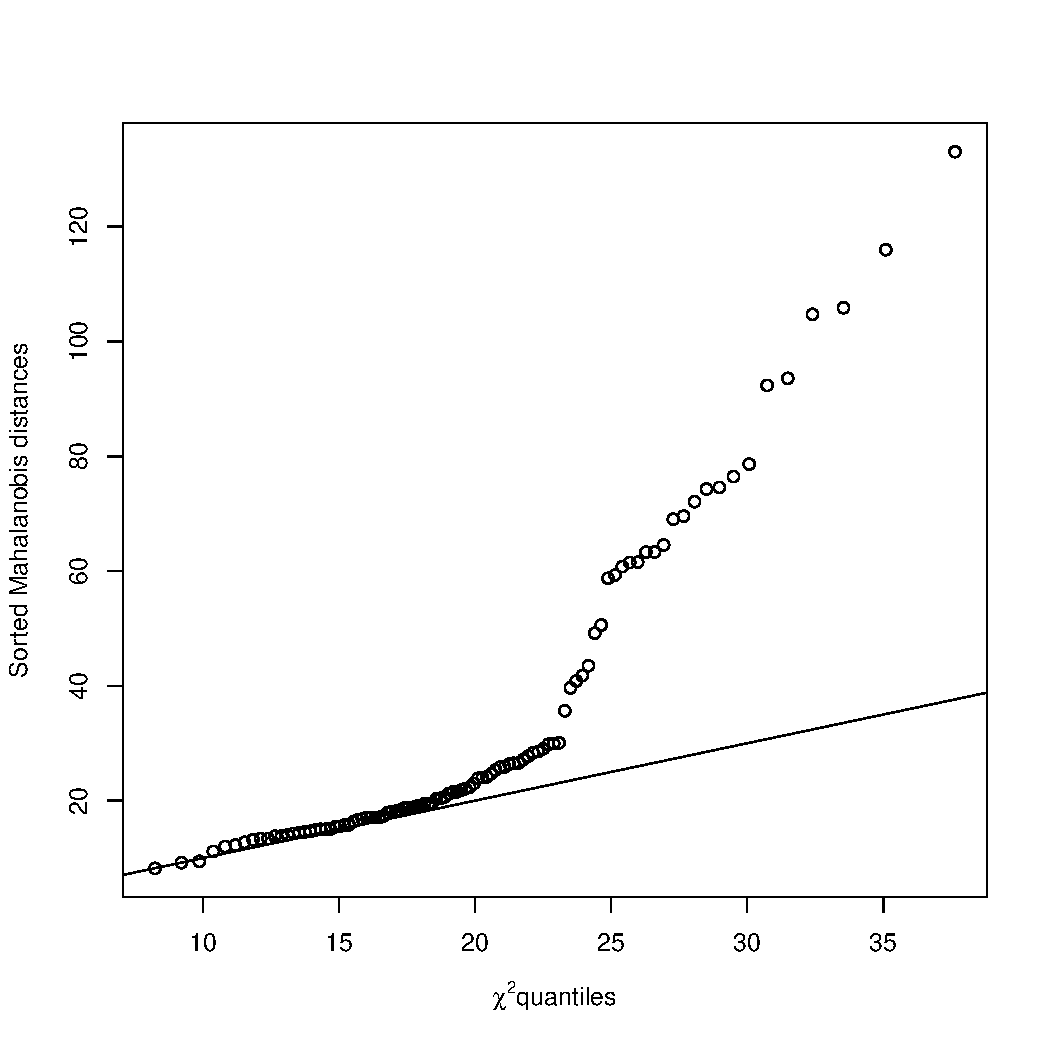
\includegraphics[width=10cm,height=10cm]{kanga.pdf}
			\caption[kg]{A mahlanobis distance graph for the kanga data set}
			\label{kanga}
		\end{figure}
		We can see some pretty extreme values. It may be worth looking into these data points. They are likely very informational
		\item f
		I was not sure what to do with this, I have a graph of the two principal components plotted against each other, but I am not sure how you would differentiate the components by sex?
		\begin{figure}[H]
			\centering
			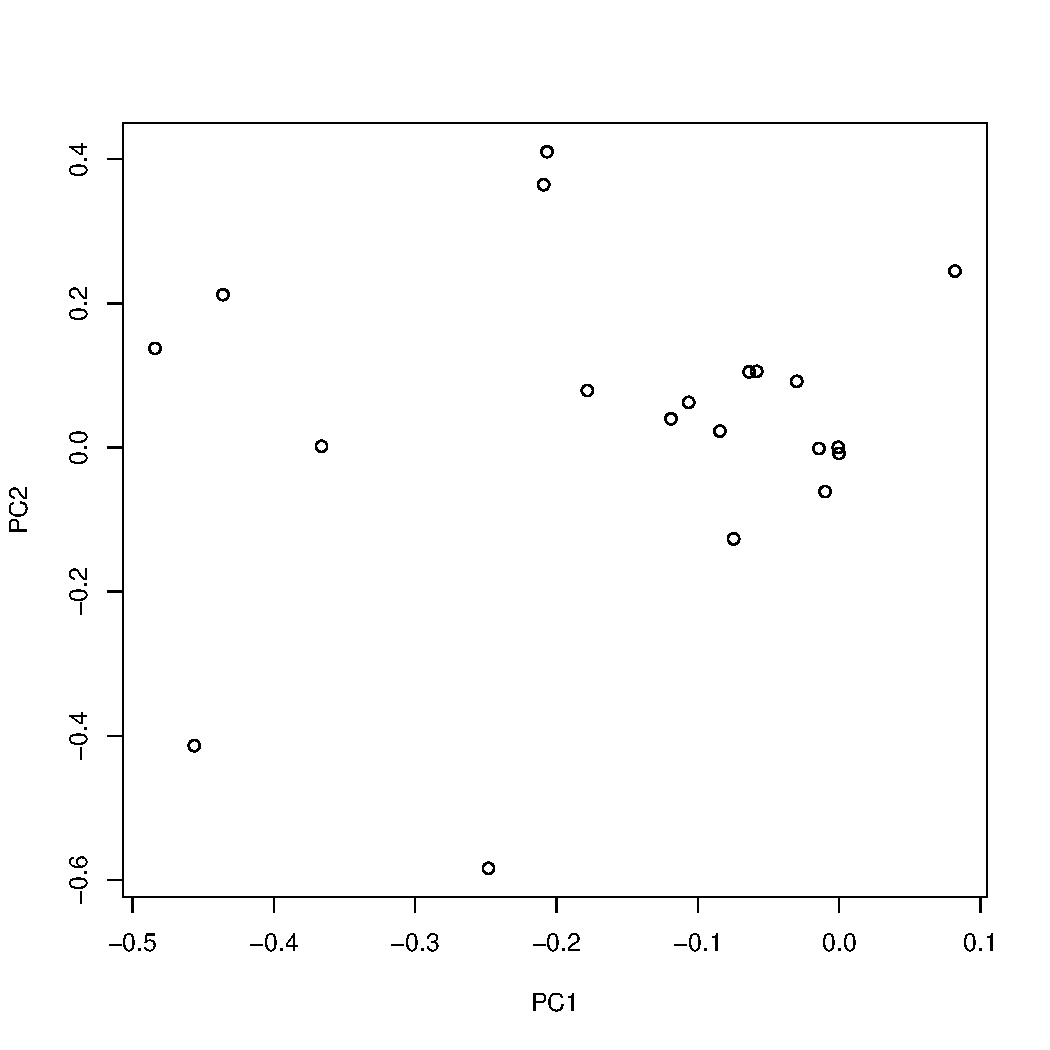
\includegraphics[width=10cm,height=10cm]{idk.pdf}
			\caption[idk]{A plot of the coefficients of PC1 against PC2}
			\label{idk}
		\end{figure}
		I suppose we can see some orthogonality / differences between components , as we would expect.
	\end{enumerate}
\end{enumerate}
\item  Finish R exercises 13.2, 13.3 of the textbook. Submit your
answers for {\color{red}ALL} questions. 
\begin{enumerate}
	\item 13.2
	\begin{enumerate}
		\item a
		\begin{verbatim}
			> glm = lm(Species~.-Endemics,gala)
			> summary(glm)
			
			Call:
			lm(formula = Species ~ . - Endemics, data = gala)
			
			Residuals:
			Min       1Q   Median       3Q      Max 
			-111.679  -34.898   -7.862   33.460  182.584 
			
			Coefficients:
			Estimate Std. Error t value Pr(>|t|)    
			(Intercept)  7.068221  19.154198   0.369 0.715351    
			Area        -0.023938   0.022422  -1.068 0.296318    
			Elevation    0.319465   0.053663   5.953 3.82e-06 ***
			Nearest      0.009144   1.054136   0.009 0.993151    
			Scruz       -0.240524   0.215402  -1.117 0.275208    
			Adjacent    -0.074805   0.017700  -4.226 0.000297 ***
			---
			Signif. codes:  0 ‘***’ 0.001 ‘**’ 0.01 ‘*’ 0.05 ‘.’ 0.1 ‘ ’ 1
			
			Residual standard error: 60.98 on 24 degrees of freedom
			Multiple R-squared:  0.7658,	Adjusted R-squared:  0.7171 
			F-statistic:  15.7 on 5 and 24 DF,  p-value: 6.838e-07
		\end{verbatim}
		Here is our simple model with a summary with the 5 geographic predictors
		\item b
		\begin{verbatim}
			> gmlm = lm(NS~Area+Anear+Dist+DistSC+Elevation,galamiss)
			> summary(gmlm)
			
			Call:
			lm(formula = NS ~ Area + Anear + Dist + DistSC + Elevation, data = galamiss)
			
			Residuals:
			Min      1Q  Median      3Q     Max 
			-114.13  -38.90  -10.03   35.34  172.19 
			
			Coefficients:
			Estimate Std. Error t value Pr(>|t|)    
			(Intercept) 17.99073   29.89638   0.602 0.555269    
			Area        -0.02700    0.02637  -1.024 0.320243    
			Anear       -0.07822    0.02159  -3.623 0.002103 ** 
			Dist        -0.09376    1.21083  -0.077 0.939182    
			DistSC      -0.29841    0.26619  -1.121 0.277857    
			Elevation    0.32213    0.06766   4.761 0.000181 ***
			---
			Signif. codes:  0 ‘***’ 0.001 ‘**’ 0.01 ‘*’ 0.05 ‘.’ 0.1 ‘ ’ 1
			
			Residual standard error: 69.17 on 17 degrees of freedom
			(6 observations deleted due to missingness)
			Multiple R-squared:  0.7636,	Adjusted R-squared:  0.6941 
			F-statistic: 10.98 on 5 and 17 DF,  p-value: 7.594e-05
		\end{verbatim}
		As we can see, missing values have reduce the number of observations available, and lowered our degrees of freedom. Our confidence has thus decreased compared to the OG.
		\item c
		\begin{verbatim}
			> gmmeans = colMeans(galamiss,na.rm = TRUE)
			> imgalamiss = galamiss
			> for(i in c(2:8)) imgalamiss[is.na(galamiss[,i]),i] <- gmmeans[i]
			> gmimlm = lm(NS~Area+Anear+Dist+DistSC+Elevation,imgalamiss)
			> summary(gmimlm)
			
			Call:
			lm(formula = NS ~ Area + Anear + Dist + DistSC + Elevation, data = imgalamiss)
			
			Residuals:
			Min     1Q Median     3Q    Max 
			-96.00 -45.43 -11.11  28.64 223.83 
			
			Coefficients:
			Estimate Std. Error t value Pr(>|t|)   
			(Intercept) -13.076462  31.291432  -0.418  0.67990   
			Area          0.000602   0.027810   0.022  0.98292   
			Anear        -0.064403   0.023002  -2.800  0.01017 * 
			Dist          0.403334   1.327801   0.304  0.76404   
			DistSC       -0.077887   0.285100  -0.273  0.78714   
			Elevation     0.269094   0.072546   3.709  0.00115 **
			---
			Signif. codes:  0 ‘***’ 0.001 ‘**’ 0.01 ‘*’ 0.05 ‘.’ 0.1 ‘ ’ 1
			
			Residual standard error: 77.03 on 23 degrees of freedom
			Multiple R-squared:  0.6382,	Adjusted R-squared:  0.5595 
			F-statistic: 8.113 on 5 and 23 DF,  p-value: 0.0001563
		\end{verbatim}
		our R squared has gone down significantly , I expect it is due to the imputated mean values to mean very little to our model and actually skew it, like we have seen in class.
		I looked at the correlation just to see if there was any to worry about.
		\begin{verbatim}
			> cor(imgalamiss)
			NS           ES       Area       Anear         Dist      DistSC     Elevation            EM
			NS         1.00000000  0.973531485  0.6162212  0.02055711 -0.019642065 -0.18622612  6.783715e-01  2.851766e-01
			ES         0.97353148  1.000000000  0.6177911  0.07370982 -0.003761533 -0.18122351  7.235296e-01  3.103206e-01
			Area       0.61622115  0.617791136  1.0000000  0.17735771 -0.114527566 -0.10897205  7.433463e-01  1.575627e-01
			Anear      0.02055711  0.073709818  0.1773577  1.00000000 -0.119674948  0.04498817  5.480544e-01  6.360495e-02
			Dist      -0.01964207 -0.003761533 -0.1145276 -0.11967495  1.000000000  0.61426960 -1.058799e-01  2.938245e-01
			DistSC    -0.18622612 -0.181223511 -0.1089720  0.04498817  0.614269601  1.00000000 -1.581337e-01  4.162295e-01
			Elevation  0.67837148  0.723529575  0.7433463  0.54805436 -0.105879903 -0.15813365  1.000000e+00 -7.548394e-18
			EM         0.28517661  0.310320605  0.1575627  0.06360495  0.293824516  0.41622947 -7.548394e-18  1.000000e+00
			> cor(galamiss)
			NS           ES       Area       Anear         Dist      DistSC Elevation         EM
			NS         1.00000000  0.973531485  0.6162212  0.02055711 -0.019642065 -0.18622612        NA 0.28517661
			ES         0.97353148  1.000000000  0.6177911  0.07370982 -0.003761533 -0.18122351        NA 0.31032061
			Area       0.61622115  0.617791136  1.0000000  0.17735771 -0.114527566 -0.10897205        NA 0.15756273
			Anear      0.02055711  0.073709818  0.1773577  1.00000000 -0.119674948  0.04498817        NA 0.06360495
			Dist      -0.01964207 -0.003761533 -0.1145276 -0.11967495  1.000000000  0.61426960        NA 0.29382452
			DistSC    -0.18622612 -0.181223511 -0.1089720  0.04498817  0.614269601  1.00000000        NA 0.41622947
			Elevation          NA           NA         NA          NA           NA          NA         1         NA
			EM         0.28517661  0.310320605  0.1575627  0.06360495  0.293824516  0.41622947        NA 1.00000000
		\end{verbatim}
		We can see that elevation is the missing data, which was our most valuable predictor in our original models. by adding mean imputated values, it has diminished the predictors ability to explain the variance in the model. There is also some correlation added by providing complete data for the model, but its not ridiculous... yet...
		\item d
		\begin{verbatim}
			> elevlm = lm(Elevation~Area+Anear+Dist+DistSC,galamiss)
			> rggalamiss=galamiss
			> galamiss[is.na(galamiss$Elevation),]
			NS ES  Area  Anear Dist DistSC Elevation EM
			Baltra       58 23 25.09   1.84  0.6    0.6        NA  0
			Coamano       2  1  0.05 903.82  1.9    1.9        NA  0
			Daphne_Major 18 11  0.34   1.84  8.0    8.0        NA  0
			Eden          8  4  0.03  17.95  0.4    0.4        NA  0
			Las_Plazas   12  9  0.23  25.09  0.5    0.6        NA  0
			Seymour      44 16  1.84  25.09  0.6    9.6        NA  0
			> rgvals = predict(elevlm,galamiss[is.na(galamiss$Elevation),])
			> sepcounter=1
			> for(i in 1:length(galamiss[,1])){
			+   if(is.na(rggalamiss[i,7]))
			+   {
			+     rggalamiss[i,7]=rgvals[sepcounter]
			+     sepcounter = sepcounter+1
			+   }
			+ }
			> rgimlm = lm(NS~Area+Anear+Dist+DistSC+Elevation,rggalamiss)
			> summary(rgimlm)
			
			Call:
			lm(formula = NS ~ Area + Anear + Dist + DistSC + Elevation, data = rggalamiss)
			
			Residuals:
			Min      1Q  Median      3Q     Max 
			-110.26  -30.88  -14.52   29.51  197.48 
			
			Coefficients:
			Estimate Std. Error t value Pr(>|t|)    
			(Intercept) -14.83873   26.26329  -0.565  0.57754    
			Area         -0.01876    0.02610  -0.719  0.47942    
			Anear        -0.07829    0.02137  -3.664  0.00129 ** 
			Dist          0.05585    1.19947   0.047  0.96326    
			DistSC       -0.09669    0.25188  -0.384  0.70459    
			Elevation     0.32213    0.06757   4.767 8.31e-05 ***
			---
			Signif. codes:  0 ‘***’ 0.001 ‘**’ 0.01 ‘*’ 0.05 ‘.’ 0.1 ‘ ’ 1
			
			Residual standard error: 69.07 on 23 degrees of freedom
			Multiple R-squared:  0.7091,	Adjusted R-squared:  0.6459 
			F-statistic: 11.21 on 5 and 23 DF,  p-value: 1.459e-05
			
		\end{verbatim}
		I wanted to see which values were missing information first. I then applied the regressed values to replace the NA points. We get a boosted performance! However, I suspect that our correlation will have increased compared to both the missing data and the mean imputated values.
		\begin{verbatim}
			> cor(rggalamiss)
			NS           ES       Area       Anear         Dist      DistSC   Elevation         EM
			NS         1.00000000  0.973531485  0.6162212  0.02055711 -0.019642065 -0.18622612  0.70180087 0.28517661
			ES         0.97353148  1.000000000  0.6177911  0.07370982 -0.003761533 -0.18122351  0.74675973 0.31032061
			Area       0.61622115  0.617791136  1.0000000  0.17735771 -0.114527566 -0.10897205  0.75415434 0.15756273
			Anear      0.02055711  0.073709818  0.1773577  1.00000000 -0.119674948  0.04498817  0.56412830 0.06360495
			Dist      -0.01964207 -0.003761533 -0.1145276 -0.11967495  1.000000000  0.61426960 -0.06913193 0.29382452
			DistSC    -0.18622612 -0.181223511 -0.1089720  0.04498817  0.614269601  1.00000000 -0.10734289 0.41622947
			Elevation  0.70180087  0.746759735  0.7541543  0.56412830 -0.069131928 -0.10734289  1.00000000 0.11884838
			EM         0.28517661  0.310320605  0.1575627  0.06360495  0.293824516  0.41622947  0.11884838 1.00000000
		\end{verbatim}
		We can see some higher correlations! As to be expected in elevation. This is always important to keep in mind
		\item e
		\begin{verbatim}
			> gm2 = galamiss[,-2]
			> gm2 = gm2[,-7]
			> mimgp = amelia(gm2,m=25)		
			> betasgp=NULL
			> sesgp=NULL
			> for(i in 1:mimgp$m)
			+ {
			+   lmod <- lm(NS~Area+Anear+Dist+DistSC+Elevation, mimgp$imputations[[i]])
			+   betasgp <- rbind(betasgp ,coef(lmod))
			+   sesgp <- rbind(sesgp ,coef(summary(lmod))[,2])
			+ }
			> (cr <- mi.meld(q=betasgp,se=sesgp))
			$q.mi
			(Intercept)        Area       Anear        Dist   DistSC Elevation
			[1,]    8.010774 -0.02177011 -0.07633469 0.004976406 -0.23399 0.3148571
			
			$se.mi
			(Intercept)       Area      Anear     Dist    DistSC  Elevation
			[1,]    22.45479 0.02413709 0.01935359 1.114134 0.2331302 0.05907911
			
			> cr$q.mi/cr$se.mi
			(Intercept)       Area     Anear        Dist    DistSC Elevation
			[1,]   0.3567512 -0.9019359 -3.944215 0.004466615 -1.003688  5.329415
		\end{verbatim}
		Looking at our coefficients P values, we can see Elevation and Anear are still the most statistically significant.
	\end{enumerate}
	\item 13.3
	\begin{enumerate}
		\item a
		\begin{verbatim}
			> pimamiss
			pregnant glucose diastolic triceps insulin  bmi diabetes age test
			1          6     148        72      35      NA 33.6    0.627  50    
			2          1      85        66      29      NA 26.6    0.351  31    
			3          8     183        64      NA      NA 23.3    0.672  32    
			4          1      89        66      23      94 28.1    0.167  21    
			5          0     137        40      35     168 43.1    2.288  33    
			6          5     116        74      NA      NA 25.6    0.201  30    
			7          3      78        50      32      88 31.0    0.248  26   
			8         10     115        NA      NA      NA 35.3    0.134  29    
			[ reached getOption("max.print") -- omitted 657 rows ]
		\end{verbatim}
		for brevity, a lot of the printouts are removed from this document. You can find the code in the R scripts. I chose not to turn 0s in pregnant and test to NAs as it makes sense for those to be zero. I did let there others turn to NAs, as we can see, insulin levels are tough to get and and are often missing. tricep is second most commonly missed, and then diastolic and bmi.
		\item b
		\begin{verbatim}
			> summary(pimalm)
			
			Call:
			lm(formula = diastolic ~ ., data = pimamiss)
			
			Residuals:
			Min      1Q  Median      3Q     Max 
			-49.420  -6.956  -0.604   7.432  29.268 
			
			Coefficients:
			Estimate Std. Error t value Pr(>|t|)    
			(Intercept) 41.004185   4.043536  10.141  < 2e-16 ***
			pregnant     0.183487   0.247575   0.741 0.459064    
			glucose      0.047134   0.025848   1.824 0.069003 .  
			triceps     -0.005719   0.074506  -0.077 0.938851    
			insulin     -0.008268   0.006027  -1.372 0.170913    
			bmi          0.532806   0.112798   4.724 3.26e-06 ***
			diabetes    -3.213760   1.722406  -1.866 0.062826 .  
			age          0.284048   0.081494   3.485 0.000548 ***
			test         0.047652   1.508849   0.032 0.974822    
			---
			Signif. codes:  0 ‘***’ 0.001 ‘**’ 0.01 ‘*’ 0.05 ‘.’ 0.1 ‘ ’ 1
			
			Residual standard error: 11.38 on 383 degrees of freedom
			(376 observations deleted due to missingness)
			Multiple R-squared:  0.1882,	Adjusted R-squared:  0.1712 
			F-statistic:  11.1 on 8 and 383 DF,  p-value: 3.94e-14
		\end{verbatim}
		poor fit, and a lot of missing data. We can see bmi and age are important, considering we are missing so much data, it doesnt seem like this model is sufficient. There seems to be some bias to the insulin levels.
		\item c
		\begin{verbatim}
			> pimameans = colMeans(pimamiss,na.rm = TRUE)
			> impimamiss = pimamiss
			> for(i in c(2:8)) impimamiss[is.na(pimamiss[,i]),i] <- pimameans[i]
			> pimaimlm =  lm(diastolic~.,impimamiss)
			> summary(pimaimlm)
			
			Call:
			lm(formula = diastolic ~ ., data = impimamiss)
			
			Residuals:
			Min      1Q  Median      3Q     Max 
			-48.879  -6.599  -0.694   6.369  56.998 
			
			Coefficients:
			Estimate Std. Error t value Pr(>|t|)    
			(Intercept) 43.205265   2.620456  16.488  < 2e-16 ***
			pregnant     0.157970   0.141327   1.118  0.26402    
			glucose      0.048453   0.016310   2.971  0.00306 ** 
			triceps      0.006457   0.054022   0.120  0.90489    
			insulin     -0.007388   0.005139  -1.438  0.15095    
			bmi          0.476441   0.071163   6.695 4.19e-11 ***
			diabetes    -2.127135   1.221251  -1.742  0.08195 .  
			age          0.285792   0.041421   6.900 1.10e-11 ***
			test        -0.868070   1.002583  -0.866  0.38686    
			---
			Signif. codes:  0 ‘***’ 0.001 ‘**’ 0.01 ‘*’ 0.05 ‘.’ 0.1 ‘ ’ 1
			
			Residual standard error: 10.92 on 759 degrees of freedom
			Multiple R-squared:  0.1938,	Adjusted R-squared:  0.1853 
			F-statistic:  22.8 on 8 and 759 DF,  p-value: < 2.2e-16
			
		\end{verbatim}
		Mean imputation provides slightly improved results in terms of R squared values. And  glucose has become very significantt. 
		\item d
		The problem described in the book didnt make sense applied to this problem. I would guess it is asking for us to regress and impute for every column and replace the NA values.
		\item e
		\begin{verbatim}
			> mimpima = amelia(pima2,m=25)
		
			> (cr <- mi.meld(q=betaspima,se=sespima))
			$q.mi
			(Intercept)  pregnant    glucose     triceps      insulin       bmi  diabetes       age       test
			[1,]     40.0757 0.1404388 0.06037759 -0.01842112 -0.008271171 0.5346332 -2.005283 0.3039374 -0.9404926
			
			$se.mi
			(Intercept)  pregnant    glucose    triceps     insulin       bmi diabetes        age     test
			[1,]    2.998815 0.1529132 0.02036614 0.06359883 0.006206634 0.0877693 1.270908 0.04602268 1.055816
			> cr$q.mi/cr$se.mi
			(Intercept) pregnant  glucose    triceps   insulin      bmi  diabetes      age      test
			[1,]    13.36384 0.918422 2.964606 -0.2896456 -1.332634 6.091347 -1.577835 6.604079 -0.890773
		\end{verbatim}
		Looking at the p values, we can see glucose,bmi, and age are quite significantt. 
	\end{enumerate}
\end{enumerate}
\item  Finish R exercises  8.1, 8.2, 8.6, of the textbook. Submit your
answers for {\color{red}ALL} questions. 
\begin{enumerate}
	\item 8.1
	\begin{enumerate}
		\item a
		\begin{figure}[H]
			\centering
			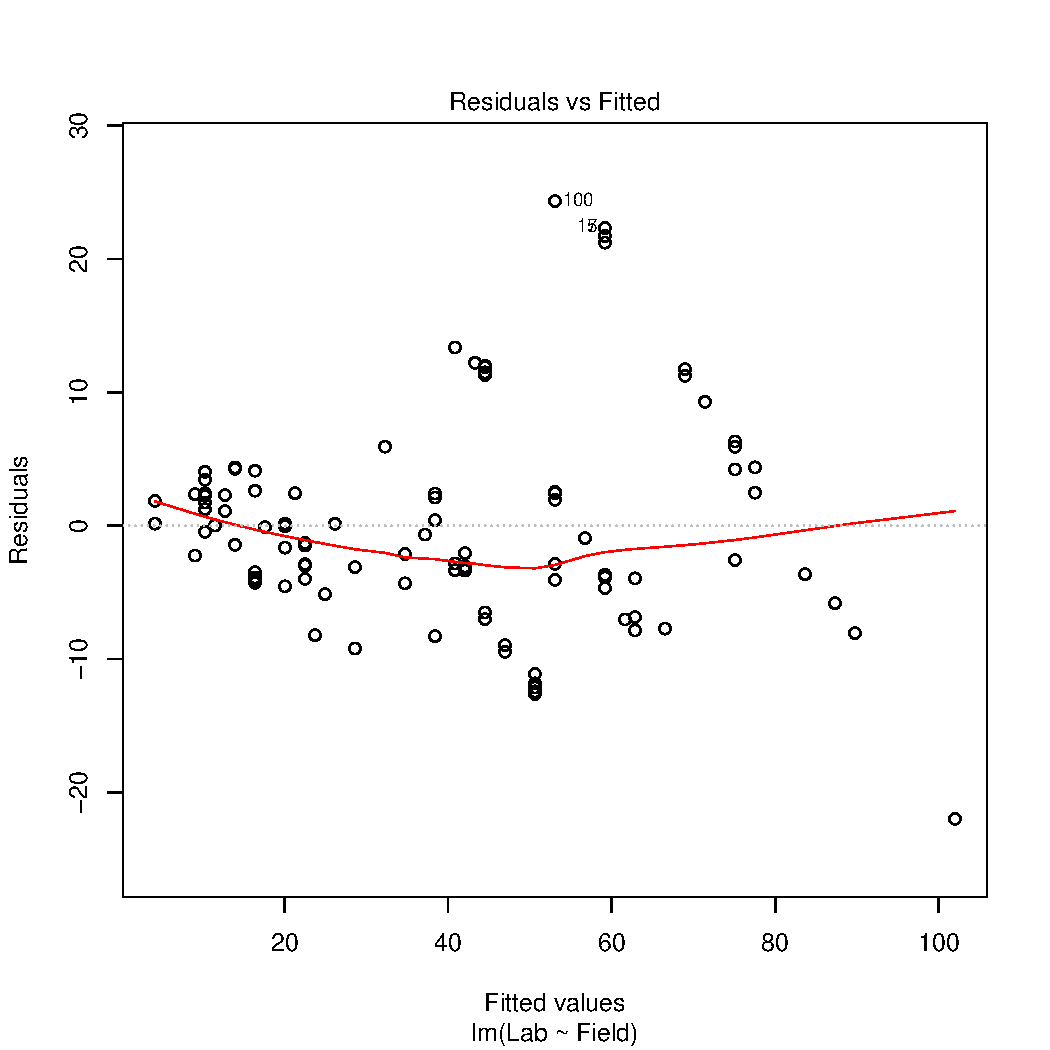
\includegraphics[width=10cm,height=10cm]{pipelinevar.pdf}
			\caption[paic]{variance check on pipeline data}
			\label{divusav}
		\end{figure}
		clearly there is some fanning here
		\item b
		\begin{verbatim}
			> summary(pipwlm)
			
			Call:
			lm(formula = Lab ~ Field, data = pipeline, weights = 1/((Field)^a_1))
			
			Weighted Residuals:
			Min      1Q  Median      3Q     Max 
			-1.7450 -0.6789 -0.2672  0.5205  2.8847 
			
			Coefficients:
			Estimate Std. Error t value Pr(>|t|)    
			(Intercept) -1.49436    0.90707  -1.647    0.102    
			Field        1.20828    0.03488  34.637   <2e-16 ***
			---
			Signif. codes:  0 ‘***’ 0.001 ‘**’ 0.01 ‘*’ 0.05 ‘.’ 0.1 ‘ ’ 1
			
			Residual standard error: 0.9795 on 105 degrees of freedom
			Multiple R-squared:  0.9195,	Adjusted R-squared:  0.9188 
			F-statistic:  1200 on 1 and 105 DF,  p-value: < 2.2e-16
		\end{verbatim}
		we see some improved R squared values as we diminish the values in order to try and prevent the fanning effect
		\item c
		\begin{figure}[H]
			\centering
			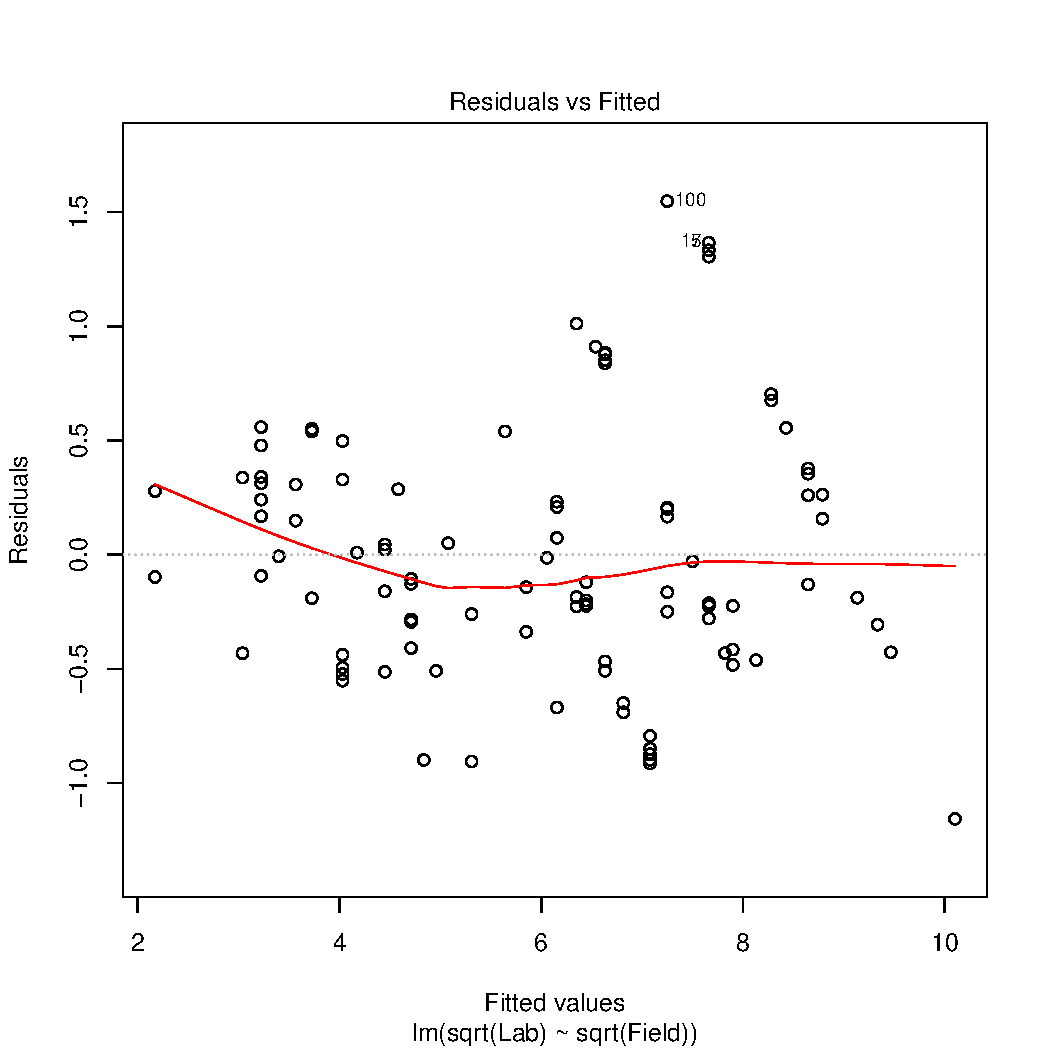
\includegraphics[width=10cm,height=10cm]{pipelinevart.pdf}
			\caption[paic]{variance check on pipeline data after transform}
			\label{divusavt}
		\end{figure}
		This is the results of taking the square root on both the response and explanatory variables. It worked quite well.
	\end{enumerate}
	\item 8.2
	\begin{enumerate}
		\item a\\
		\begin{figure}[!htb]
			\begin{minipage}{0.48\textwidth}
				\centering
				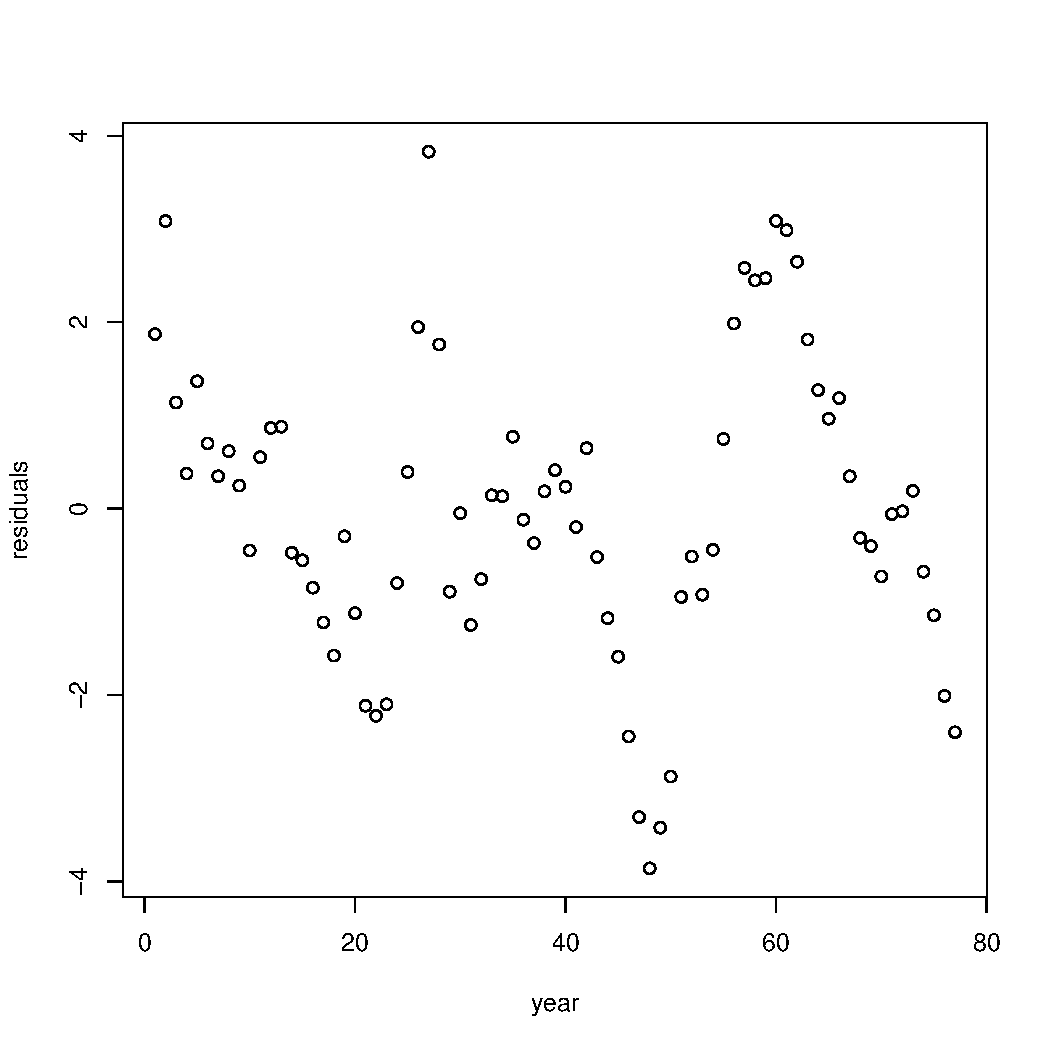
\includegraphics[width=.7\linewidth]{ovtusa.pdf}
				\caption{looking at the error correlation of divusa }\label{Fig:Data1}
			\end{minipage}
			\begin {minipage}{0.48\textwidth}
			\centering
			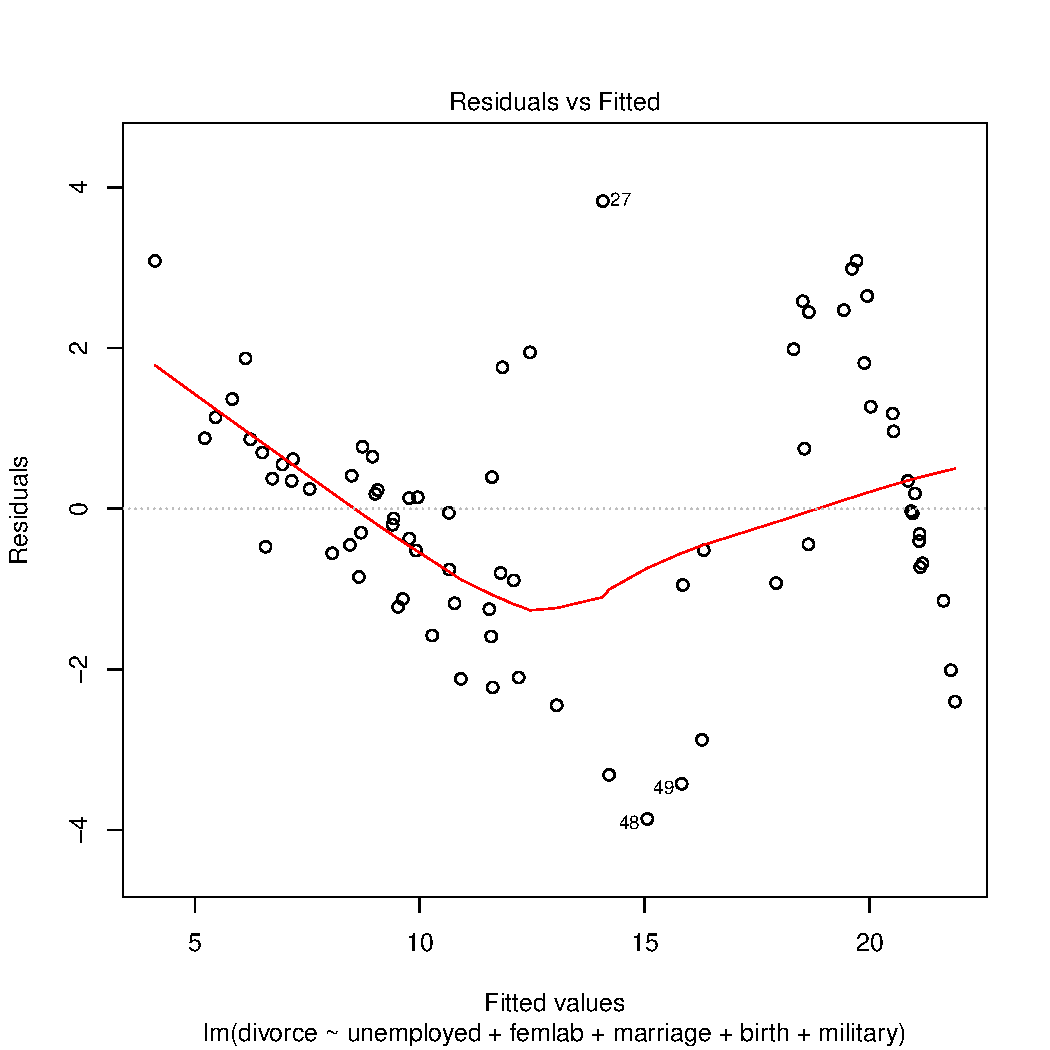
\includegraphics[width=.7\linewidth]{duse1.pdf}
			\caption{Another look at error correlation of divusa}\label{Fig:Data2}
			\end{minipage}
		\end{figure}
		we can see there is a correlation over time between the residuals/errors
		\item b
		\begin{verbatim}
			> summary(glusalm)
			Generalized least squares fit by maximum likelihood
			Model: divorce ~ unemployed + femlab + marriage + birth + military 
			Data: divusa 
			AIC      BIC    logLik
			179.9523 198.7027 -81.97613
			
			Correlation Structure: AR(1)
			Formula: ~year 
			Parameter estimate(s):
			Phi 
			0.9715486 
			
			Coefficients:
			Value Std.Error   t-value p-value
			(Intercept) -7.059682  5.547193 -1.272658  0.2073
			unemployed   0.107643  0.045915  2.344395  0.0219
			femlab       0.312085  0.095151  3.279878  0.0016
			marriage     0.164326  0.022897  7.176766  0.0000
			birth       -0.049909  0.022012 -2.267345  0.0264
			military     0.017946  0.014271  1.257544  0.2127
			
			Correlation: 
			(Intr) unmply femlab marrig birth 
			unemployed -0.420                            
			femlab     -0.802  0.240                     
			marriage   -0.516  0.607  0.307              
			birth      -0.379  0.041  0.066 -0.094       
			military   -0.036  0.436 -0.311  0.530  0.128
			
			Standardized residuals:
			Min         Q1        Med         Q3        Max 
			-1.4509327 -0.9760939 -0.6164694  1.1375377  2.1593261 
			
			Residual standard error: 2.907665 
			Degrees of freedom: 77 total; 71 residual
			> intervals(glusalm,which="var-cov")
			Approximate 95% confidence intervals
			
			Correlation structure:
			lower      est.     upper
			Phi 0.6528097 0.9715486 0.9980192
			attr(,"label")
			[1] "Correlation structure:"
			
			Residual standard error:
			lower       est.      upper 
			0.7974404  2.9076645 10.6020628 
		\end{verbatim}
		we can see that unemployed has become significant, in the previous model, the pvalue was higher.
		\\
		Further their correlation is significant, we see a positive correlation with a confidence interval that is quite strong
		\item c
		Personally, I believe these are correlated over the years mainly due to the warts the data set covers. Baby boomers are all likely to get married around the same time, and thus divorce in similar times as well. Further, War usually causes couples to get married just before leaving for service or after. Thus when they return they will realize they werent meant to be and similarly get divorced at similar times. 
	\end{enumerate}
	\item 8.6
	\begin{enumerate}
		\item a
		\begin{figure}[H]
			\centering
			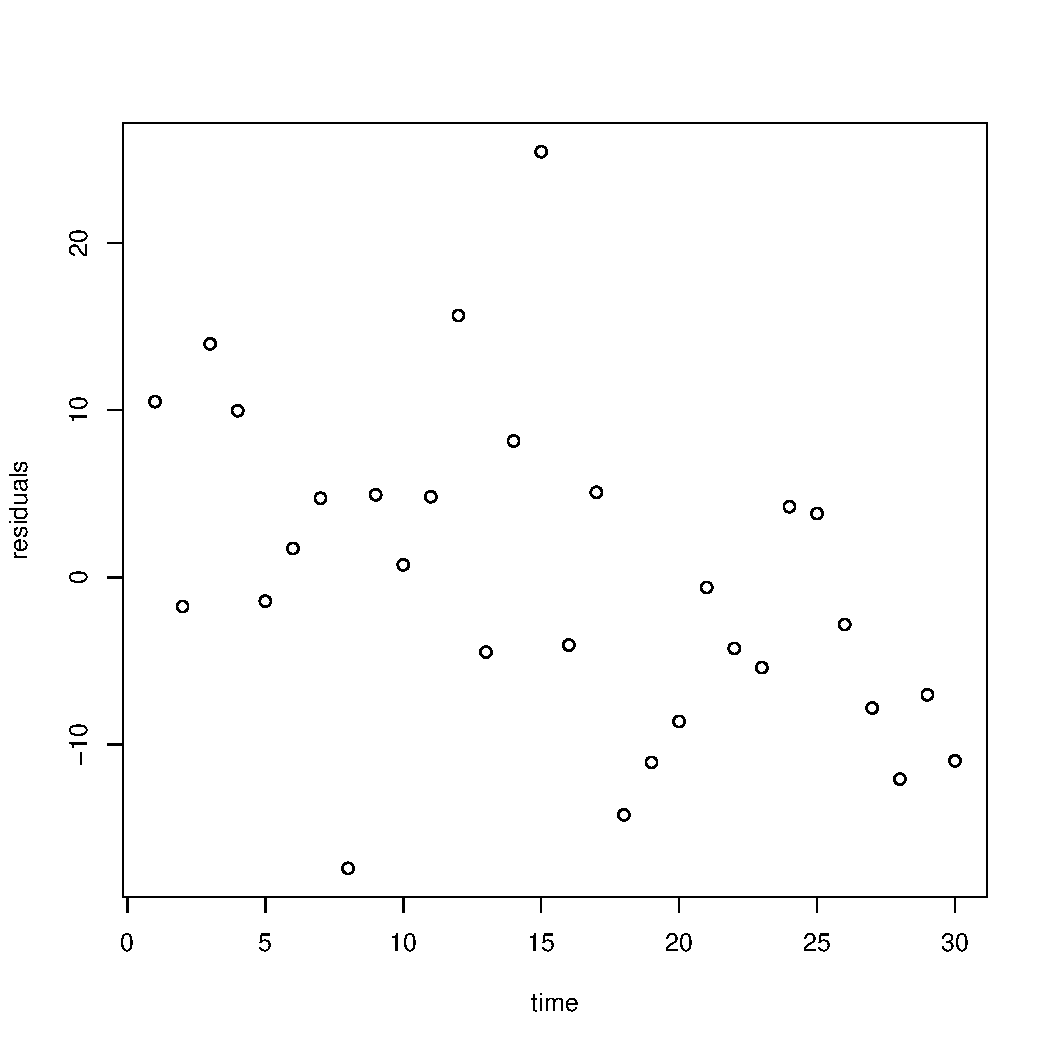
\includegraphics[width=10cm,height=10cm]{ovtc.pdf}
			\caption[paic]{we can see a somehwat linear trend over time that is decreasing.}
			\label{ovtc}
		\end{figure}
		Not a strong indicator, but something
		\item b
		\begin{verbatim}
			Generalized least squares fit by REML
			Model: taste ~ . - time 
			Data: c2 
			AIC      BIC  logLik
			214.94 222.4886 -101.47
			
			Correlation Structure: AR(1)
			Formula: ~time 
			Parameter estimate(s):
			Phi 
			0.2641944 
			
			Coefficients:
			Value Std.Error   t-value p-value
			(Intercept) -30.332472 20.273077 -1.496195  0.1466
			Acetic        1.436411  4.876581  0.294553  0.7707
			H2S           4.058880  1.314283  3.088284  0.0047
			Lactic       15.826468  9.235404  1.713674  0.0985
			
			Correlation: 
			(Intr) Acetic H2S   
			Acetic -0.899              
			H2S     0.424 -0.395       
			Lactic  0.063 -0.416 -0.435
			
			Standardized residuals:
			Min          Q1         Med          Q3         Max 
			-1.64546468 -0.63861716 -0.06641714  0.52255676  2.41323021 
			
			Residual standard error: 10.33276 
			Degrees of freedom: 30 total; 26 residual
			> intervals(cgls,which="var-cov")
			Approximate 95% confidence intervals
			
			Correlation structure:
			lower      est.     upper
			Phi -0.1690265 0.2641944 0.6118599
			attr(,"label")
			[1] "Correlation structure:"
			
			Residual standard error:
			lower     est.    upper 
			7.62646 10.33276 13.99940 
		\end{verbatim}
		We can see that the confidence interval include 0, and thus we can not really trust this correlation.
		\item 
		\begin{verbatim}
			> clm2 = lm(taste~.,c2)
			> summary(clm2)
			
			Call:
			lm(formula = taste ~ ., data = c2)
			
			Residuals:
			Min       1Q   Median       3Q      Max 
			-22.3523  -4.9735  -0.5089   4.8531  23.1311 
			
			Coefficients:
			Estimate Std. Error t value Pr(>|t|)   
			(Intercept) -36.6127    17.9845  -2.036  0.05250 . 
			Acetic        4.1275     4.2556   0.970  0.34139   
			H2S           3.5387     1.1315   3.127  0.00444 **
			Lactic       17.9527     7.7875   2.305  0.02973 * 
			time         -0.5459     0.2043  -2.672  0.01306 * 
			---
			Signif. codes:  0 ‘***’ 0.001 ‘**’ 0.01 ‘*’ 0.05 ‘.’ 0.1 ‘ ’ 1
			
			Residual standard error: 9.112 on 25 degrees of freedom
			Multiple R-squared:  0.7291,	Adjusted R-squared:  0.6858 
			F-statistic: 16.83 on 4 and 25 DF,  p-value: 8.205e-07
		\end{verbatim}
		Unlike the GLS, our OLS thinks time is significant! Very funny. However, this is not contradictory, LS and GLS are quite different. This is explained in the next part.
		\item d \\ in the GLS, we are looking at how correlated the error or noise is over "time", or consecutive entries unlike our ordinary LS. Within the OLS the time value is being included to see how it may provide information on our response. The difference lies within the relations. In OLS it changes the significance and value based on a linear combination within each entry. In residuals, we are only considering the impact of the time variable \textbf{AFTER} the coefficients have been established
		\item e\\if i was told that the entries were not in chronological order, then this would make it purely coincidental that consecutive entries are related, and we should randomize their order to avoid the seemingly correlated entries
	\end{enumerate}
\end{enumerate}
\end{enumerate}

\end{document}
